\documentclass[aspectratio=169,11pt]{beamer}
% ==========================================================================
%  KSA lecture-slide theme  =  stock beamer "Boadilla"  +  KSA colour theme
%  brand colours sampled from the official KSA symbol mark:
%    Deep Prussian Blue  #2E3192   (지성 - intellect)
%    Golden Gray         #D6CBB1   (감성 - sensibility)
%  Engine: XeLaTeX.  Usage:
%    \documentclass[aspectratio=169,11pt]{beamer}
%    \input{../../theme/ksa-theme.tex}
%  Each deck lives in its own slides/kor/<deck>/ folder together with its
%  own images; ../../figs/ is kept only as a fallback for the shared cache.
% ==========================================================================

\usepackage{fontspec}
\usepackage{amsmath,amssymb}
\usepackage{graphicx}
\graphicspath{{figs/}{./}{../../../figs/}}
\usepackage{booktabs}
\usepackage{listings}
\usepackage{varwidth}

% ---- fonts (no ctex/xeCJK on this box -> fontspec drives CJK directly) -----
\defaultfontfeatures{Ligatures=TeX}
\setmainfont{Noto Sans CJK KR}
\setsansfont{Noto Sans CJK KR}
\setmonofont{Noto Sans Mono CJK KR}[Scale=0.92]

% ---- base theme: stock Boadilla ------------------------------------------
\usetheme{Boadilla}
\usefonttheme{professionalfonts}
\setbeamertemplate{navigation symbols}{}

% ---- KSA colour theme (recolour the stock theme) --------------------------
\definecolor{ksablue}{HTML}{2E3192}
\definecolor{ksabluedk}{HTML}{20226A}
\definecolor{ksagold}{HTML}{D6CBB1}
\definecolor{ksagolddk}{HTML}{A9976B}
\definecolor{ksared}{HTML}{C0392B}
\definecolor{ksagray}{HTML}{5B5B5B}

\setbeamercolor{structure}{fg=ksablue}
\setbeamercolor{alerted text}{fg=ksared}

\setbeamercolor{palette primary}{fg=white,           bg=ksablue}
\setbeamercolor{palette secondary}{fg=white,         bg=ksablue!85!black}
\setbeamercolor{palette tertiary}{fg=white,          bg=ksabluedk}
\setbeamercolor{titlelike}{fg=ksablue}
\setbeamercolor{frametitle}{fg=ksablue,bg=}
\setbeamercolor{title}{fg=ksablue}
\setbeamercolor{author}{fg=ksagray}
\setbeamercolor{institute}{fg=ksagray}
\setbeamercolor{block title}{fg=white,bg=ksablue}
\setbeamercolor{block body}{fg=black!85,bg=ksablue!6}
\setbeamercolor{item}{fg=ksablue}
\setbeamercolor{section in toc}{fg=black!85}

\setbeamerfont{frametitle}{series=\bfseries}
\setbeamerfont{title}{series=\bfseries}

% ---- footline:  KSA mark | "Made by ..." | n / N   (matches reference) ----
\newcommand{\ksacredit}{}
\setbeamertemplate{footline}{%
  \hbox{%
    \begin{beamercolorbox}[wd=.18\paperwidth,ht=2.6ex,dp=1.5ex,leftskip=1.1em]{}%
      \raisebox{-0.35ex}{\includegraphics[height=2.0ex]{ksa-logo.png}}%
    \end{beamercolorbox}%
    \begin{beamercolorbox}[wd=.64\paperwidth,ht=2.6ex,dp=1.5ex,center]{}%
      {\scriptsize\color{ksagray}\ksacredit}%
    \end{beamercolorbox}%
    \begin{beamercolorbox}[wd=.18\paperwidth,ht=2.6ex,dp=1.5ex,rightskip=1.1em]{}%
      \hfill{\scriptsize\color{ksablue}\insertframenumber\,/\,\inserttotalframenumber}%
    \end{beamercolorbox}%
  }%
  \vskip2pt
}

% ---- section divider: stock \sectionpage, KSA-coloured -------------------
\setbeamertemplate{section page}{%
  \begingroup\centering
    {\color{ksagolddk}\rule{0.16\paperwidth}{1pt}}\par\vskip1.0em
    {\usebeamerfont{title}\color{ksablue}\insertsectionhead\par}\vskip1.0em
    {\color{ksagolddk}\rule{0.16\paperwidth}{1pt}}\par
  \endgroup
}
\AtBeginSection[]{\begin{frame}[plain,noframenumbering]\vfill\sectionpage\vfill\end{frame}}

% ---- code listings ------------------------------------------------------------
\lstdefinestyle{ksa}{%
  basicstyle=\ttfamily\scriptsize,
  keywordstyle=\color{ksablue}\bfseries,
  commentstyle=\color{ksagray}\itshape,
  stringstyle=\color{ksagolddk},
  numberstyle=\tiny\color{ksagray},
  backgroundcolor=\color{ksablue!6},
  frame=leftline, framerule=1.4pt, rulecolor=\color{ksablue},
  xleftmargin=1em, aboveskip=0.8em, belowskip=0.4em,
  showstringspaces=false, breaklines=true, language=Python,
}
\lstset{style=ksa}

% ---- handy macros -----------------------------------------------------------
\newcommand{\kb}[1]{\textbf{\color{ksablue}#1}}   % blue keyword
\newcommand{\kq}[1]{\textbf{\color{ksared}#1}}    % red key-question

\setbeamerfont{title}{series=\bfseries,size=\fontsize{24}{30}\selectfont}
\setbeamerfont{subtitle}{series=\bfseries,size=\fontsize{14}{18}\selectfont}
\setbeamerfont{author}{size=\normalsize}
\setbeamerfont{institute}{size=\small}
\graphicspath{{figs/}{../../../../assets/}}
\makeatletter
\newcommand{\markpage}[1]{\protected@write\@auxout{}{\string\newlabel{#1}{{\the\c@framenumber}{}}}\hypertarget{#1}{}}
\newcommand{\pref}[1]{\hyperlink{#1}{\textcolor{ksagolddk}{(p.\ref{#1})}}}
\makeatother

\renewcommand{\ksacredit}{Machine Learning 1 \,\textperiodcentered\, 어텐션}
\title{어텐션 (Attention)}
\subtitle{비슷한 만큼 섞어 온다}
\author{Machine Learning 1}
\institute{한국과학영재학교 (KSA)}
\date{}
\begin{document}
\begin{frame}[plain,noframenumbering]\titlepage\end{frame}


% --- 오늘의 질문
\begin{frame}{오늘의 질문: ``그것은'' 은 무엇일까?}
\vfill
\centering
{\LARGE 동물은 도로를 건너지 않았다. \kb{그것은} 너무 피곤했다.}\vskip1em
{\large 사람은 바로 안다: 그것은 = \textcolor{ksablue}{동물} \quad (``너무 넓었다'' 였다면 = 도로)}\\[0.6em]
{\large AI 는 단어마다 \textbf{어느 단어를 얼마나 볼지} 정해야 한다 \quad $\to$ \textbf{어텐션}}
\vfill
\note{동물은 도로를 건너지 않았다. 그것은 너무 피곤했다. 여기서 그것은 무엇일까요? 사람은 바로 동물이라고 압니다. 만약 그것은 너무 넓었다였다면 도로겠죠. AI가 이걸 알려면, 그것은이라는 단어를 이해할 때 다른 단어 중 어느 단어를 얼마나 볼지 정해야 합니다. 이걸 정하는 방법이 오늘 배울 어텐션입니다.}
\end{frame}

% --- 시작: Seq2Seq 의 병목
\begin{frame}{시작: Seq2Seq 의 벡터 하나를 벗어나기}
\markpage{idea}
\vfill
\centering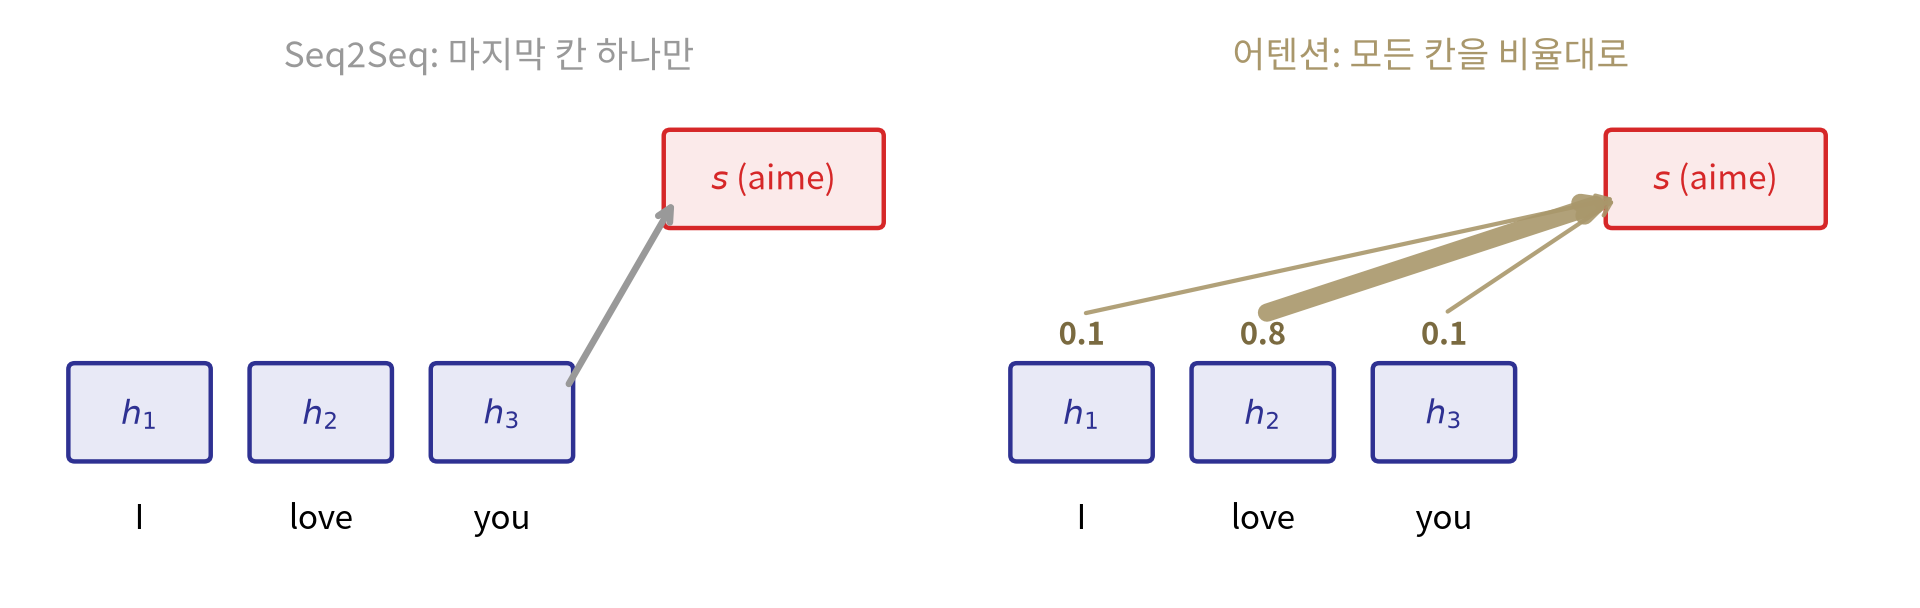
\includegraphics[width=0.86\linewidth]{at_idea.png}\par\vskip0.2em
{\large 디코더가 단어를 쓸 때마다 인코더의 \kb{모든 칸}을 다시 보고, 필요한 칸을 더 많이 섞는다}\\[0.2em]
{\small Bahdanau, Cho, Bengio (2014) \quad 섞는 비율도 학습으로 정해진다}
\vfill
\note{어텐션은 지난 시간 Seq2Seq의 한계에서 시작했습니다. Seq2Seq의 디코더는 인코더의 마지막 칸, 벡터 하나만 봤습니다. 2014년 바다나우, 조경현, 벤지오는 디코더가 단어를 쓸 때마다 인코더의 모든 칸을 다시 보고, 필요한 칸을 더 많이 섞어 오게 했습니다. aime를 쓸 때는 love 칸을 0.8, 나머지를 0.1씩 섞는 식입니다. 이 비율은 사람이 정하지 않고 학습으로 정해집니다.}
\end{frame}

% --- 도서관 비유
\begin{frame}{도서관 비유: Query · Key · Value}
\vfill
\centering
\renewcommand{\arraystretch}{1.7}
{\large\begin{tabular}{lll}
\textcolor{ksared}{Query} $\mathbf{q}$ & 내 질문 & 지금 단어가 찾는 것\\
\textcolor{ksablue}{Key} $\mathbf{k}_j$ & 책마다 붙은 색인 카드 & 각 단어가 ``나는 이런 단어'' 라고 내건 것\\
\textcolor{ksagolddk}{Value} $\mathbf{v}_j$ & 책 내용 & 실제로 가져올 정보
\end{tabular}}\vskip0.8em
{\large 질문을 모든 색인 카드와 비교 $\to$ 비슷할수록 높은 비율 $\to$ 그 비율대로 내용을 섞어 온다}
\vfill
\note{어텐션은 도서관에 비유하면 이해하기 쉽습니다. 내 질문을 쿼리, 책마다 붙은 색인 카드를 키, 책 내용을 밸류라고 합니다. 쿼리를 모든 키와 비교해서, 비슷할수록 높은 비율을 주고, 그 비율대로 밸류를 섞어 옵니다. 책 한 권만 고르는 게 아니라 여러 책을 비율대로 섞는다는 점이 중요합니다. Seq2Seq 번역에서는 디코더의 메모가 쿼리, 인코더의 칸들이 키이자 밸류였습니다.}
\end{frame}

% --- 식
\begin{frame}{식으로}
\markpage{formula}
\vfill
\centering
\renewcommand{\arraystretch}{1.6}
{\Large\begin{tabular}{rl}
점수 & $e_j = \dfrac{\mathbf{q} \cdot \mathbf{k}_j}{\sqrt{d}}$ \qquad (내적: 비슷할수록 크다)\\
비율 & $\alpha_j = \text{softmax}(e)_j = \dfrac{\exp(e_j)}{\sum_i \exp(e_i)}$ \qquad (합이 1)\\
결과 & $\mathbf{z} = \sum_j \alpha_j \mathbf{v}_j$
\end{tabular}}\vskip0.6em
{\large 여러 단어를 한꺼번에: \quad $\text{Attention}(Q, K, V) = \text{softmax}\!\left(\dfrac{Q K^\top}{\sqrt{d}}\right) V$}\\[0.2em]
{\small $d$: 벡터 칸 수 \quad 이 꼴 (scaled dot-product) 은 트랜스포머 논문 (Vaswani 외 2017)}
\vfill
\note{식으로 쓰면 세 줄입니다. 점수는 쿼리와 키의 내적을 벡터 칸 수 d의 제곱근으로 나눈 값입니다. 방향이 비슷할수록 내적이 큽니다. 점수를 softmax에 넣으면 합이 1인 비율 알파가 됩니다. 결과는 밸류들을 알파 비율로 더한 벡터 z입니다. 여러 단어의 쿼리를 행렬 Q로 모으면 한 줄로, softmax Q K 전치 나누기 루트 d 곱하기 V로 쓸 수 있습니다. 이 꼴은 2017년 트랜스포머 논문에서 나왔습니다.}
\end{frame}

% --- 손 계산
\begin{frame}{손으로 한 번: ``그것은'' 이 보는 곳}
\markpage{hand}
\vfill
\begin{columns}[c]
\column{0.42\linewidth}\centering
\renewcommand{\arraystretch}{1.25}
{\large\begin{tabular}{lc}
단어 & 벡터 (예시)\\\hline
동물 & (3, 0, 0)\\
도로 & (0, 3, 0)\\
건너지 & (0, 0, 3)\\
\kb{그것은} & (2.8, 0.3, 0)
\end{tabular}}\\[0.4em]
{\small Q = K = V = 이 벡터 \quad $d = 3$}
\column{0.56\linewidth}\centering
점수 $= \mathbf{q}_{\text{그것은}} \cdot \mathbf{k} / \sqrt{3}$\\[0.2em]
동물 $8.4 / 1.73 = \kb{4.85}$ \quad 도로 0.52 \quad 건너지 0\\
자기 자신 $(7.84 + 0.09) / 1.73 = 4.58$\\[0.4em]
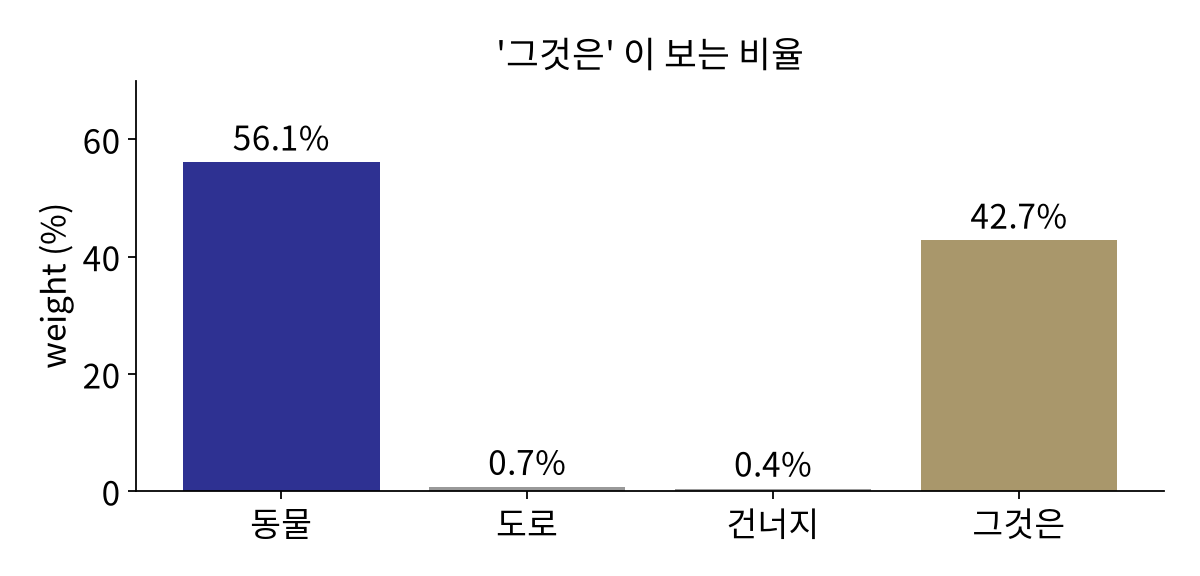
\includegraphics[width=0.85\linewidth]{at_it.png}
\end{columns}\vskip0.3em
\centering{\large 새 벡터 $= 0.561 \cdot$ 동물 $+ \cdots = \kb{(2.88, 0.15, 0.01)}$ \quad $\approx$ 동물 (3, 0, 0)}
\vfill
\note{직접 계산해 봅시다. 단어 벡터는 그것은이 동물과 비슷하도록 직접 만든 3칸짜리 예시이고, 쿼리, 키, 밸류를 모두 이 벡터로 둡니다. 그것은의 쿼리와 동물의 키를 내적하면 2.8 곱하기 3, 8.4이고, 루트 3, 1.73으로 나누면 4.85입니다. 도로는 0.9를 나눠 0.52, 건너지는 0, 자기 자신은 4.58입니다. softmax에 넣으면 동물 56퍼센트, 자기 자신 43퍼센트, 도로와 건너지는 1퍼센트도 안 됩니다. 이 비율로 밸류를 섞은 새 벡터는 2.88, 0.15, 0.01, 거의 동물 벡터입니다. 그것은의 새 표현에 동물의 뜻이 들어간 겁니다.}
\end{frame}

% --- 왜 루트 d
\begin{frame}{왜 $\sqrt{d}$ 로 나누나}
\vfill
\centering
{\large 칸마다 평균 0, 분산 1 인 무작위 벡터의 내적: \quad 분산 $= d$, \quad 표준편차 $= \sqrt{d}$}\vskip0.6em
\renewcommand{\arraystretch}{1.4}
{\large\begin{tabular}{lcc}
 & $d = 3$ & $d = 512$\\\hline
내적의 표준편차 & 1.7 & \kq{22.6}\\
$\sqrt{d}$ 로 나누면 & 1 & 1
\end{tabular}}\vskip0.8em
{\large 점수가 수십이면 softmax 가 0 아니면 1 \quad $\to$ 한 단어만 보고 기울기도 0 근처}\\[0.3em]
{\large $\sqrt{d}$ 로 나눠 점수의 크기를 칸 수와 상관없이 맞춘다}
\vfill
\note{왜 루트 d로 나눌까요? 칸마다 평균 0, 분산 1인 무작위 벡터 두 개를 내적하면, d개 곱을 더하니 분산이 d, 표준편차가 루트 d입니다. d가 3이면 1.7이지만, 트랜스포머처럼 512칸이면 22.6입니다. 점수가 수십씩 차이 나면 softmax가 거의 0 아니면 1이 되어 한 단어만 보게 되고, 기울기도 거의 0이 되어 학습이 안 됩니다. 그래서 루트 d로 나눠 칸 수와 상관없이 점수의 크기를 1 정도로 맞춥니다.}
\end{frame}

% --- 실험: 베끼기
\begin{frame}{실험: Seq2Seq 에 어텐션을 더하면}
\markpage{exp}
\vfill
\centering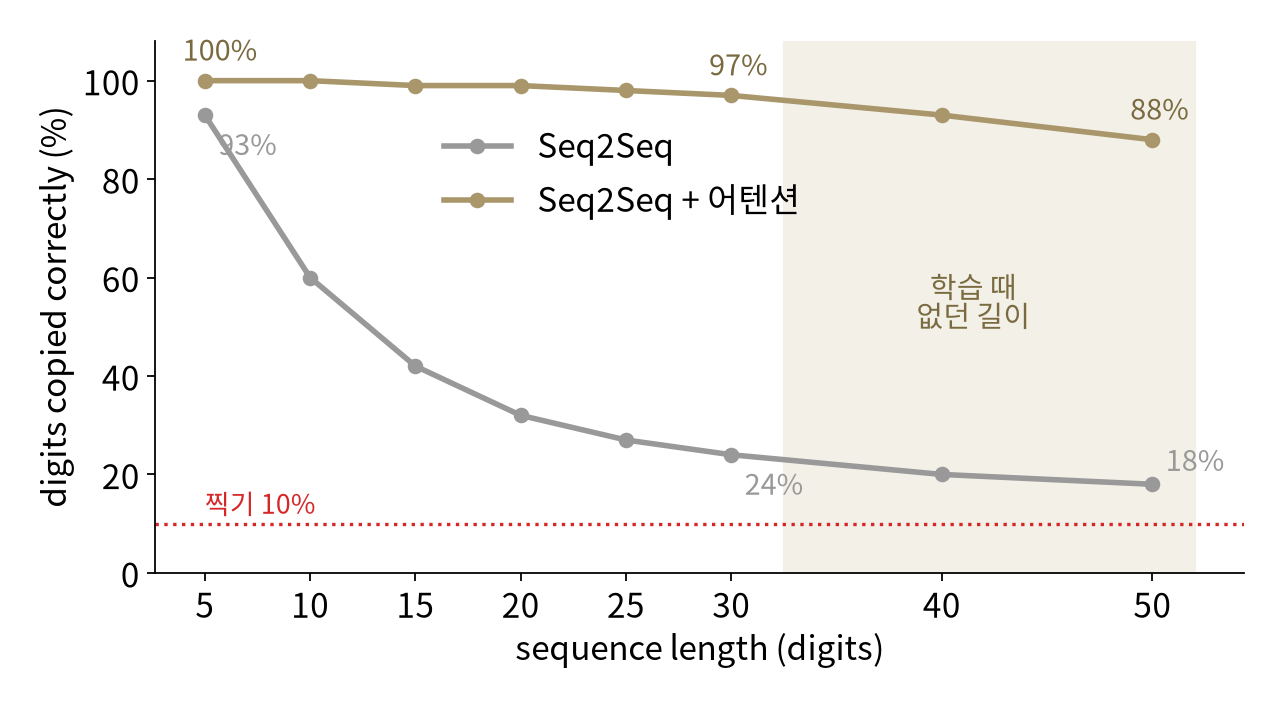
\includegraphics[width=0.58\linewidth]{at_copy.png}\par\vskip0.2em
{\large 지난 시간의 숫자열 베끼기 (벡터 32칸) \quad 길이 30: \kq{24\%} $\to$ \kb{97\%}}\\[0.2em]
{\large 학습 때 없던 길이 50 도 88\% \quad 통째로 맞힌 비율 (길이 30): 0\% $\to$ 92\%}
\vfill
\note{지난 시간의 숫자열 베끼기 실험에 어텐션만 더해 봤습니다. 벡터 크기 32, 학습 걸음 수, 모두 같습니다. 어텐션 없이는 길이 30에서 숫자의 24퍼센트만 맞혔는데, 어텐션을 더하니 97퍼센트입니다. 학습 때는 길이 30까지만 봤는데, 처음 보는 길이 40은 93퍼센트, 50도 88퍼센트입니다. 숫자열을 통째로 맞힌 비율은 길이 30에서 0퍼센트에서 92퍼센트가 됐습니다. 이제 정보가 벡터 하나를 지나갈 필요가 없으니까요. 참고로 지난 시간에 도움이 됐던 입력 거꾸로 넣기는, 어텐션이 있으면 오히려 나빴습니다. 길이 30에서 63퍼센트였습니다.}
\end{frame}

% --- 어텐션 지도
\begin{frame}{어텐션 지도: 어디를 봤나}
\vfill
\begin{columns}[c]
\column{0.46\linewidth}\centering
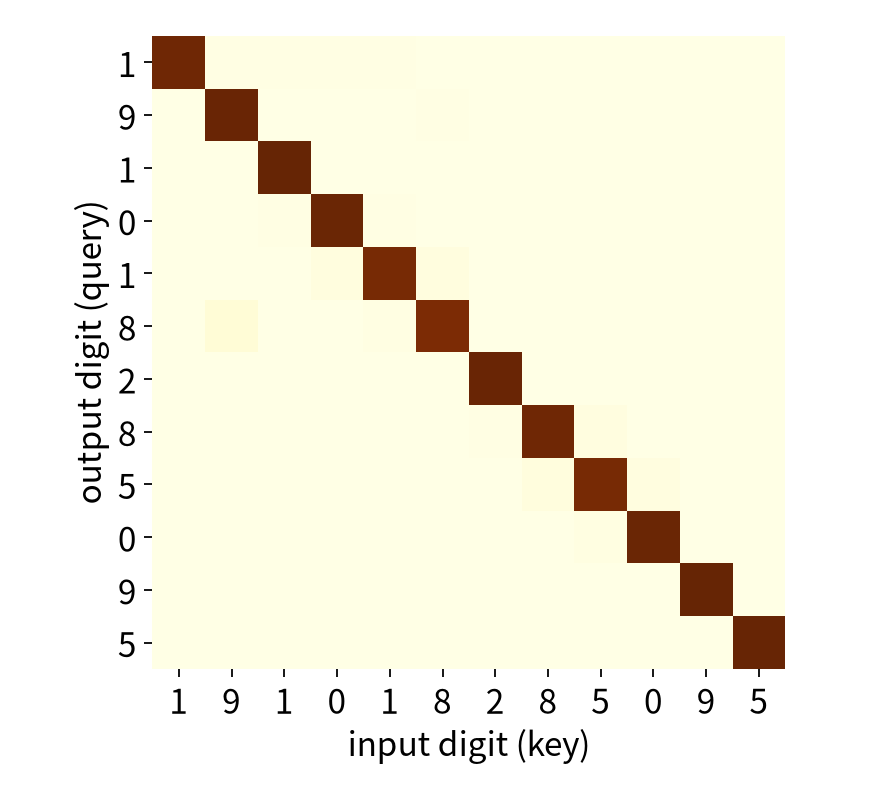
\includegraphics[width=\linewidth]{at_map.png}
\column{0.5\linewidth}
{\large 칸 = 출력 숫자 (행) 가 입력 숫자 (열) 를 보는 비율 $\alpha$}\\[0.8em]
{\large \kb{대각선}: $k$ 번째 숫자를 쓸 때 $k$ 번째 입력을 본다}\\[0.8em]
{\large 시키지 않았는데 스스로 배웠다}\\[0.8em]
{\small 번역에서는 어순이 다른 곳에서 대각선이 꺾인다 (Bahdanau 외 2014 그림 3: 영어 European Economic Area $\leftrightarrow$ 프랑스어 zone économique européenne)}
\end{columns}
\vfill
\note{어텐션의 좋은 점은 모델이 어디를 봤는지 볼 수 있다는 겁니다. 길이 12 숫자열을 베낄 때의 비율 알파를 그렸습니다. 행이 출력 숫자, 열이 입력 숫자입니다. 정확히 대각선입니다. k번째 숫자를 쓸 때 k번째 입력을 거의 100퍼센트 봅니다. 어디를 보라고 알려 준 적이 없는데 스스로 배운 겁니다. 실제 번역에서는 어순이 다른 곳에서 대각선이 꺾입니다. 바다나우 논문의 그림에서 영어 European Economic Area가 프랑스어 zone économique européenne으로, 순서가 거꾸로 대응되는 게 보입니다.}
\end{frame}

% --- 셀프 어텐션
\begin{frame}{번역의 보조에서 주인공으로}
\vfill
\centering
\renewcommand{\arraystretch}{1.6}
{\large\begin{tabular}{lll}
2014 & Bahdanau 외 & RNN 번역에 어텐션: BLEU 17.8 $\to$ \kb{26.8}\\
2015 & Luong 외 & 점수를 내적으로 (오늘 실험의 방식)\\
2017 & Vaswani 외 & \textbf{셀프 어텐션}만으로 트랜스포머
\end{tabular}}\vskip0.6em
\renewcommand{\arraystretch}{1.3}
{\large\begin{tabular}{ll}
번역 (교차) 어텐션 & Q = 디코더, K · V = 인코더\\
\textbf{셀프} 어텐션 & Q · K · V 모두 같은 문장 \quad (``그것은'' 예)
\end{tabular}}
\vfill
\note{어텐션은 번역 RNN의 보조로 시작했습니다. 2014년 바다나우 논문에서, 길이 50까지의 문장으로 학습한 영어 프랑스어 번역의 BLEU가 17.8에서 26.8로 올랐습니다. 2015년 루옹은 점수를 내적으로 계산하는 더 간단한 방법을 썼고, 오늘 실험이 이 방식입니다. 2017년 트랜스포머는 Attention Is All You Need라는 제목처럼 RNN을 빼고 셀프 어텐션만으로 만들었습니다. 번역 어텐션은 쿼리가 디코더, 키와 밸류가 인코더에서 오지만, 셀프 어텐션은 셋 다 같은 문장에서 옵니다. 오늘 그것은 예제가 바로 셀프 어텐션입니다. 다음 시간에 트랜스포머를 배웁니다.}
\end{frame}

% --- 문제풀이
\begin{frame}{문제풀이}
\vfill
\begin{enumerate}
\item 점수가 (2, 0, 0) 이면 비율 $\alpha$ 는? ($e^2 \approx 7.39$) \quad 밸류가 (10), (0), (0) 이면 결과는?\vskip0.8em
\item 손 계산에서 ``그것은'' 벡터를 (0.3, 2.8, 0) 으로 바꾸면 어느 단어를 가장 많이 볼까?\vskip0.8em
\item 입력 단어 $n$ 개, 출력 단어 $m$ 개인 번역에서 점수는 몇 개 계산하나? Seq2Seq 와 비교하면?\vskip0.8em
\item 실험에서 어텐션 모델은 학습 때 없던 길이 50 도 88\% 맞혔다. Seq2Seq 는 왜 못할까?
\end{enumerate}
\vfill
\note{1번 답. 7.39, 1, 1을 더하면 9.39이니 비율은 약 0.79, 0.11, 0.11이고, 결과는 7.9입니다. 2번 답. 이번엔 도로와 비슷하니 도로를 가장 많이 봅니다. 3번 답. 출력 단어마다 입력 n개와 비교하니 m 곱하기 n개입니다. Seq2Seq는 이런 비교가 없는 대신 벡터 하나에 모든 걸 담아야 했습니다. 4번 답. Seq2Seq는 길이 50의 정보를 벡터 32칸에 담아야 하지만, 어텐션은 쓸 때마다 해당 칸을 직접 찾아 보니 길이가 길어져도 덜 무너집니다.}
\end{frame}

% --- 실습
\begin{frame}{실습}
\vfill
\centering\begin{tabular}{rl}
\large 1 & numpy 로 어텐션 함수 $\to$ ``그것은'' 손 계산 (56\% · 43\%), $\sqrt{d}$ 실험\\[0.5em]
\large 2 & Seq2Seq 에 어텐션 더하기 (PyTorch) $\to$ 숫자열 베끼기 길이별 정답률\\[0.5em]
\large 3 & 어텐션 지도 그리기
\end{tabular}\vskip1em
\href{https://colab.research.google.com/github/SuminHan/book-ml/blob/main/slides/v2/ml1/week12/attention/lab/attention.ipynb}{\textcolor{ksagolddk}{▶ Colab에서 실습 노트북 열기}}
\vfill
\note{실습은 세 부분입니다. 첫째, numpy로 어텐션 함수를 만들어 그것은 손 계산을 재현하고, 루트 d로 나누지 않으면 어떻게 되는지 봅니다. 둘째, 지난 시간의 Seq2Seq에 어텐션을 더해 숫자열 베끼기 정답률을 길이별로 잽니다. 셋째, 어텐션 지도를 그려 모델이 어디를 보는지 확인합니다.}
\end{frame}

% --- 정리
\begin{frame}{정리}
\vfill
\centering\large\begin{tabular}{l}
\textbf{어텐션}: 질문 (Q) 을 모든 색인 (K) 과 비교 $\to$ softmax 비율 $\to$ 내용 (V) 을 섞는다\\[0.5em]
$\text{softmax}(QK^\top / \sqrt{d})\,V$ \quad $\sqrt{d}$: 칸이 많아도 점수 크기를 맞춘다\\[0.5em]
``그것은'' $\to$ 동물 56\% \quad 베끼기 길이 30: 24\% $\to$ \kb{97\%}, 지도는 대각선\\[0.5em]
2014 번역의 보조 $\to$ 2017 셀프 어텐션만으로 트랜스포머 (다음 시간)
\end{tabular}
\vfill
\note{정리합니다. 어텐션은 쿼리를 모든 키와 비교해 softmax로 비율을 만들고, 그 비율대로 밸류를 섞어 옵니다. 식은 softmax Q K 전치 나누기 루트 d 곱하기 V이고, 루트 d는 칸이 많아도 점수 크기를 맞춰 줍니다. 그것은은 동물을 56퍼센트 봤고, 숫자열 베끼기는 길이 30에서 24퍼센트가 97퍼센트가 됐으며, 어텐션 지도는 대각선이었습니다. 2014년 번역의 보조로 시작한 어텐션은 2017년 트랜스포머의 전부가 됩니다. 다음 시간에 배웁니다.}
\end{frame}
\end{document}
